%!TEX program = xelatex
% 完整编译: xelatex -> biber/bibtex -> xelatex -> xelatex
\documentclass[lang=cn,a4paper,newtx]{elegantpaper}

\title{InfSup 条件学习笔记}
\author{陈春雨 \\ 湘潭大学\ 数学与计算科学学院}

\date{\today}

\begin{document}

\maketitle

\begin{abstract}
在偏微分方程理论以及偏微分方程数值解方法的稳定性分析中,我们经常会遇到 InfSup 条件,
其形式为:
$\inf_{u\in U}\sup_{v\in V}\frac{a(u, v)}{\|u\|_V\|v\|_Q}\geq \beta > 0$
本文将会讨论 InfSup 条件与稳定性之间的关系。理解 InfSup 条件的关键在于
1. 连续映射不一定把闭集映射成闭集。
2. InfSup 条件等价于某个算子的像空间是闭的。
本文主要内容是基于 Long Chen 教授的课程笔记加上自己的一些理解。
\end{abstract}

\section{泛函分析的一些知识}
\begin{enumerate}
\item \textbf{Riesz 表示定理:}Hilbert 空间 $V$ 中的元素 $u$ 唯一对应于 $V'$ 
    中的一个线性泛函 $f$, 使得:
    $$ 
    f(v) = (u, v)_{V} 
    $$ 
    记 $u^* = f = R_Vu$, $f_* = u = R_V^{-1}f$。

\item $U$ 是一个 Hilbert 空间,$V \subseteq U$ 是 $U$ 的一个子空间,那么
    $V^{\perp}$ 是闭的。
    \begin{proof}
        令 $\{u_k\}$ 是 $V^{\perp}$ 中的一组柯西收敛列,那么根据 $H$ 是 Hilbert
        空间可知 $\{u_k\}$ 收敛于 $U$ 中的元素 $u$, 对于任意 $v \in V$,
        $$
        (u_k, v) = 0
        $$
        所以:
        $$
        0 = \lim_{k\to\infty}(u_k, v) = \lim_{k\to\infty}v^*(u_k) =
        v^*(\lim_{k\to\infty} u_k) = v^*(u) = (u, v)
        $$
        所以 $u \in V^{\perp}$,因此 $V^{\perp}$ 是闭的。
    \end{proof}

\item \textbf{Banach 定理:} $U$ 和 $V$ 是两个 Banach 空间,$f$ 是 $U$ 到 $V$
    的有界线性算子,且 $f$ 是一个双射,那么 $f$ 存在逆映射 $f^{-1}$, 而且 $f^{-1}$
    也是有界的。

\item 对于连续映射 $f$, 一个开集(闭集)的原象还是开集(闭集),但是一个开集(闭集)
    的象不一定是开集(闭集)。

\item \textbf{什么算子的像空间是闭的?} 首先我们考虑连续 $U$ 到 $V$有界算子,
    因为 $A(\mathrm{Ker}(A))=0$ 是闭的,所以我们只需要证明
    $A(U/\mathrm{Ker}(A))$ 是闭的,所以我们默认 $A$ 是单射。然后看如下公式:
    $$
    \|Au_k-Au_m\|\leq \|A\|\|u_k-u_m\|
    $$
    那么 $Au_k$ 是柯西列不能得到 $u_k$ 是柯西列!我们需要让不等式反向!
    即 
    $$
    C\|u_k-u_m\|\leq \|Au_k-Au_m\|
    $$
    上式可以推出 $A$ 是单射。在有限维的情况下,上式和 $A$
    是单射等价,但是在无限维空间中不等价。所以满足上式的算子像空间是闭的。

\item \textbf{Hahn-Banach 定理:} $U$ 是一个范数线性空间,
    $M$ 是 $U$ 的一个子空间,
    $f: M \to \mathbb{R}$ 是一个 $M$ 上的一个有界线性泛函,那么 $f$ 可以延拓到
    $U$ 上, 且 $\|f\|_{U'} = \|f\|_{M'}$。
    \begin{note}
        两个重要的推论:
        \begin{enumerate}
            \item 若 $S$ 是范数线性空间 $U$ 的一个子空间,$v\in U, v\notin S$,
                那么存在 $f\in U'$ 使得 $f|_S = 0$ 且 $f(v) = 1$。
            \item 若 $U$ 是一个范数线性空间那么 $\forall v \in U$,
                存在 $f\in U'$ 使得 $\|f\|_{U'} = \|v\|$ 且 $f(v) = \|v\|_U$。 
        \end{enumerate}
        其中第一的推论可以用于证明 $U$ 的某个子空间 $S$ 是闭的,假设 $S$ 不是闭的,
        那么存在 $v\in \bar{S}\backslash S$,根据推论一,存在 $f\in U'$ 使得
        $f|_S = 0$ 且 $f(v) = 1$,根据这个条件结合实际情况可以得到矛盾。
        第二个推论类似与 Riesz 表示定理。
    \end{note}

\item 对于一个映射 $A: U \to V$,可以定义 $A$ 的图像 $\Gamma(A)$:
        $$
        \Gamma(A) = \{(u, Au): u\in U\}
        $$
        $\Gamma(A)$ 是 $U\times V$ 的子空间。对 $\Gamma(A)$ 定义范数:
        $$
        \|(u, Au)\|_{U\times V} = \|u\|_U + \|Au\|_V
        $$
        那么当 $\Gamma(A)$ 是闭的时候,称 $A$ 是闭的。

\item \textbf{闭算子定理:} 假设 $U, V$ 是 Banach 空间,$A: U \to V$ 是一个线性算子,
    那么 $A$ 是闭的当且仅当 $A$ 是连续的。
    \begin{note}
        本文中所有的算子 $A : U\to V$ 都表示其定义域是 $U$,值域不一定是 $V$。
        当 $A$ 的定义域是 $U$ 的子集时,如果 $A$ 是无界算子那么 $A$ 的定义域
        至多在 $A$ 中是稠密的。
    \end{note}
    

\item 对于一个 $U\times V$ 上的双线性型 $b$,存在 $B \in \mathcal{L}(U, V')$ :
    $$
    b(u, v) = \langle Bu,  v\rangle_{V'\times V}
    $$
    同时 $B^T\in \mathcal{L}(V, U')$:
    $$
    b(u, v) = \langle u,  B^Tv\rangle_{U\times U'}
    $$
    $B^T$ 称为 $B$ 的共轭算子或简称 $B$ 的转置. 有以下结论:
    $$
    \mathrm{Ker}(B) = \mathrm{Im}(B^T)^0, \quad 
    \mathrm{Ker}(B^T) = \mathrm{Im}(B)^0
    $$

\item 根据上面的定义可以重写 InfSup 条件:
    $$
    \inf_{v\in V}\sup_{q\in Q}\frac{b(v, q)}{\|v\|_V\|q\|_Q} \geq \beta > 0
    $$
    为:
    $$
    \inf_{v\in V}\sup_{q\in Q}\frac{\langle Bv,  q\rangle}{\|v\|_V\|q\|_Q} \geq
    \beta > 0
    $$

\item \textbf{闭像定理:} 以下三个条件等价:
    \begin{enumerate}
        \item $\mathrm{Im}(B)$ 是闭的。
        \item $\mathrm{Im}(B) = \mathrm{Ker}(B^T)^0$。
        \item 存在 $L_B : \mathrm{Im}(B) \to \mathrm{Ker}(B)^{\perp}$ 满足: 
            $$
            B(L_Bv) = v, \quad \forall v \in \mathrm{Im}(B)
            $$
            且存在 $\beta > 0$:
            $$
            \beta\|L_Bv\| \leq \|v\|, \quad \forall v \in \mathrm{Im}(B) 
            $$
    \end{enumerate} 
    $B$ 换成 $B^T$ 一样成立。
    \begin{note}
        第三个条件成立等价于 
        $$
        \beta\|u\|_{U} \leq \|Bu\|_{U'}, \quad \forall u \in \mathrm{Ker}(B)^{\perp}
        $$
    \end{note}


\item $\mathrm{Im}(B)$ 闭当且仅当 $\mathrm{Im}(B^T)$ 闭。
    \begin{proof}
        若 $\mathrm{Im}(B)$ 闭,那么存在一个 $L_B$ 是 $B$ 的右逆,
        那么对于任意 $v \in \mathrm{Ker}(B^T)^{\perp}$, 
        $$
        \|v\|^2 = (v, v)_V = \langle BL_BR_Vv,  v\rangle =
        \langle L_BR_Vv,  B^T v\rangle \leq \|L_BR_Vv\|\|B^Tv\| 
        \leq \beta^{-1}\|B^Tv\|\|v\|
        $$
        所以 
        $$
        \|v\| \leq \beta^{-1}\|B^Tv\|
        $$
        \begin{figure}[h]
            \centering
            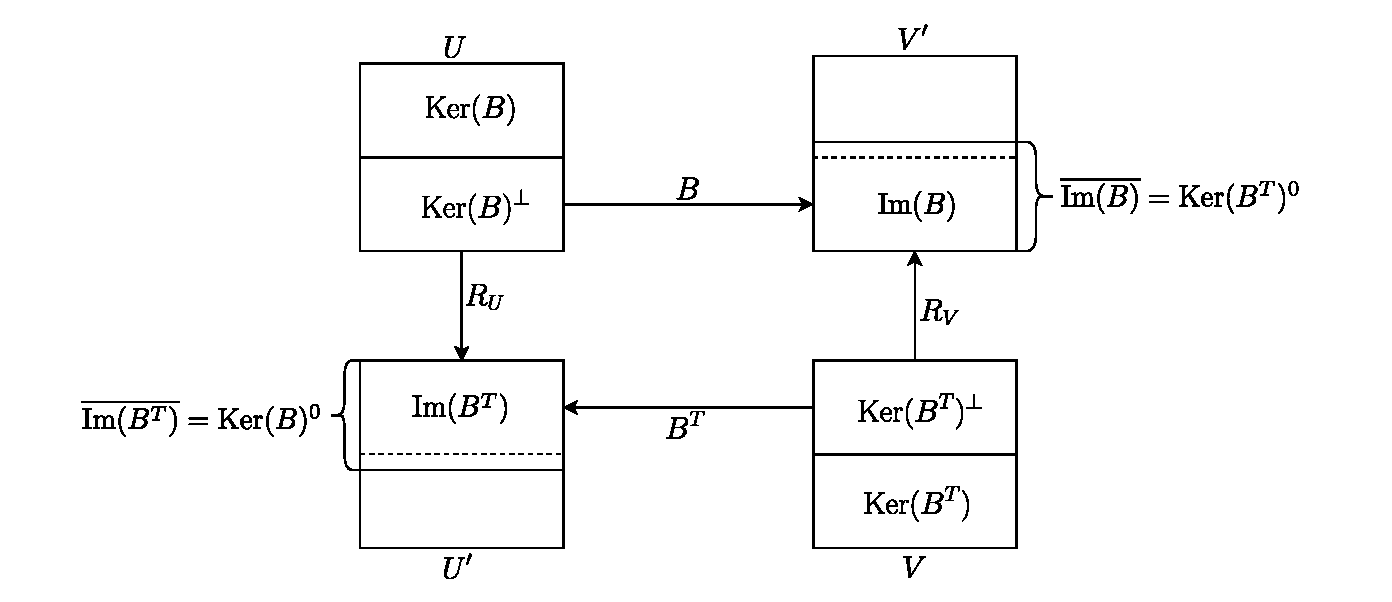
\includegraphics[width=0.8\textwidth]{../figures/operator.pdf}
            \caption{算子 $B$ 和 $B^T$ 的空间对应}
        \end{figure}
        这满足第三个条件,所以 $\mathrm{Im}(B^T)$ 闭。
    \end{proof}

\end{enumerate}

\section{Babu\v{s}ka 理论}
现在考虑一个算子方程 $Au = f$ 的适定性问题。其中 $A: U \to V^*$
是一个有界线性算子,$U, V$ 是 Banach 空间。

首先考虑解的唯一性问题,解的唯一性等价与 $A$ 是单射,有以下定理:

\begin{theorem}
    $A$ 是单射且 $\mathrm{Im}(A)$ 闭的充要条件是存在 $\beta > 0$ 使得:
    $$
    \beta\|u\|_U \leq \|Au\|_V, \quad \forall u \in U
    $$
\end{theorem}
\begin{proof}
    \textbf{必要性}:因为 $\mathrm{Im}(A)$ 是闭的,所以其继承 $V$ 的范数结构后是一个
    Banach 空间,根据 Banach 定理存在 线性有界算子 $A^{-1} : \mathrm{Im}(A) \to U$
    所以 $\forall u \in U$
    $$
    \|u\|_U = \|A^{-1}(Au)\|_U \leq \|A^{-1}\| \|Au\|_V
    $$
    令 $\beta = \|A^{-1}\|^{-1}$ 不等式成立。

    \textbf{充分性}:若不等式成立,那么当 $Au = 0$ 那么根据不等式可知 $u = 0$,
    所以 $A$ 是单射。对于任意柯西列 $\{A u_k\}_{k=0}^{\infty} \subset
    \mathrm{Im}(A)$ 根据不等式可知 $\{u_k\}_{k=0}^{\infty}$ 同样是柯西列,所以存在
    $u \in U$, $\lim_{k\to\infty} u_k = u$,所以根据 $A$ 的连续性 $Au_k$ 收敛于
    $Au$。
\end{proof}

所以当 $A$ 有下界时,解的唯一性问题得到解决。接下来考虑解的存在性问题,
简单来说解的存在性问题就是 $A$ 的像空间就是 $V$,即 $A$
是满射。满射性可以用其对偶算子 $A^T$ 的单射有下界来描述:
\begin{theorem}
    \label{thm:surjection}
    令 $U, V$ 是 Banach 空间,$A: U \to V$ 是一个有界线性算子,那么 $A$ 是满射的
    充要条件是 $A^T$ 是单射且 $\mathrm{Im}(A^T)$ 是闭的。
\end{theorem}
\begin{proof}
    \textbf{必要性}:因为 $A$ 是满射,所以 $\mathrm{Im}(A) = V'$,
    当 $A^T v = 0$,根据 Hahn-Banach 定理,存在
    $v^* \in V'$ 使得 $\|v\| = \|v^*\|, v^*(v) = \|v\|^2$,根据 $A$ 是满射,
    可知存在 $u \in U$ 使得 $Au = v^*$,
    $$
    \|v\|^2 = \langle v^*,  v\rangle = \langle Au,  v\rangle 
    = \langle u,  A^Tv\rangle
    (Au,  v)_V = (u,  A^Tv)_U = 0
    $$
    所以 $v = 0$,所以 $A^T$ 是单射。根据闭像定理,$\mathrm{Im}(A^T)$ 是闭的。

    \textbf{充分性}:若 $A$ 不是满射,那么存在 $v \in V$ 使得 $v \notin \mathrm{Im}(A)$,
    根据 Hahn-Banach 定理,存在 $f\in V'$ 使得 $f|_{\mathrm{Im}(A)} = 0$ 且 $f(v) = 1$,
    $(A^T f_*, u)_U = (f_*, Au) = f(Au) = 0$,
    所以 $A^T f_* = 0$,而 $A^T$ 是单射,所以 $f_* = 0$,所以 $f = 0$,矛盾。
    所以 $A$ 是满射。
\end{proof}

最后一个是解的稳定性问题,即要求:
$$
\|u\|_U \leq C\|f\|_V
$$
显然这等价与 $A$ 有下界。所以 $Au = f$ 的适定性问题等价于 $A$ 有下界,
且 $A^T$ 有下界。

\subsection{应用于变分问题}
令 $a(u, v)$ 是 $U\times V$ 上的一个双线性型,满足:
\begin{align}
\label{upboundofa}
a(u, v) \leq \beta\|u\|_U\|v\|_V
\end{align}
$f\in V'$ 是 $V$ 上的一个连续线性泛函,考虑如下变分问题:
\begin{align}
\label{var0}
a(u, v) = f(v), \quad \forall v \in V
\end{align}
我们可以定义 $A: U \to V'$:
$$
\langle Au,  v\rangle = a(u, v), \quad \forall v \in V
$$
那么 $A^T: V \to U'$ 定义如下:
$$
\langle A^T v,  u\rangle = a(u, v), \quad \forall u \in U
$$
问题 \eqref{var0} 可以修改为: 对于 $f \in V'$, 求解 $u \in U$ 使得:
$$
Au = f
$$
根据前面的讨论,问题的适定性等价于 $A$ 有下界且 $A^T$ 有下界。即存在 $\alpha, \beta > 0$:
$$
\alpha\|u\|_U \leq \|Au\|_{V'}, \quad \beta\|v\|_V \leq \|A^Tv\|_{U'}
$$
根据对偶算子范数的定义,上面的式子等价于:
$$
\alpha\|u\|_U \leq \sup_{v\in V}\frac{ \langle Au,  v\rangle}{\|v\|_V} = 
\sup_{v\in V}\frac{a(u, v)}{\|v\|_V}, \quad
\beta\|v\|_V \leq \sup_{u\in U}\frac{ \langle A^Tv,  u\rangle}{\|u\|_U} =
\sup_{u\in U}\frac{a(u, v)}{\|u\|_U}
$$
即如下的 InfSup 条件:
\begin{align}
\label{infsupconditiona}
\inf_{u\in U}\sup_{v\in V}\frac{a(u, v)}{\|u\|_U\|v\|_V} \geq \alpha > 0, \quad
\inf_{v\in V}\sup_{u\in U}\frac{a(u, v)}{\|u\|_U\|v\|_V} \geq \beta > 0
\end{align}
总结为如下定理:
\begin{theorem}
    \label{thm:wellposednessa}
    令 $a(u, v)$ 满足 \eqref{upboundofa},且存在 $\alpha, \beta > 0$ 满足
    \eqref{infsupconditiona},那么对于任意 $f\in V'$,问题 \eqref{var0} 存在唯一解。
    进一步的,当 \eqref{infsupconditiona} 成立时:
    $$
    \alpha = \beta = \|A^{-1}\| = \|A^{-T}\|
    $$
\end{theorem}

注意 InfSup 条件 \eqref{infsupconditiona} 等价于如下两个条件:
\begin{itemize}
    \item 对于任意 $v\in V$,存在 $u\in U$ 使得:
        $$
        a(u, v)\geq C \|u\|_U\|v\|_V
        $$
    \item 对于任意 $u\in U$,存在 $v\in V$ 使得:
        $$
        a(u, v)\geq C \|u\|_U\|v\|_V
        $$
\end{itemize}
以第一个条件为例,$v$ 到 $u$ 的映射实际上是连续的,如下:
\begin{corollary}
    若 $a(u, v)$ 满足 \eqref{upboundofa},那么存在 $\alpha > 0$ 满足
    \eqref{infsupconditiona}第一个不等式等价于:对于任意 $v\in V$,存在 $u\in U$ 使得:
    $$
    a(u, v)\geq C_1 \|v\|_U\|v\|_V
    $$
    且
    $$
    \|u\|_U \leq C_2\|v\|_V
    $$
\end{corollary}
\begin{proof}
    充分性显然,必要性: 令 $v\in V$,那么存在 $f \in V'$ 使得 $f(v) = \|v\|_V^2$,
    $\|f\| = \|v\|$,根据 $A$ 是满射,可知存在 $u \in U$ 使得 $Au = f$,那么
    $$
    \|u\|_U = C\|f\|_U = C\|v\|_V
    $$
    且
    $$
    a(u, v) = \langle Au,  v\rangle = f(v) = \|v\|_V^2
    $$
    必要性得证。
\end{proof}

当 $U = V$ 时,上面的 InfSup 条件等价于 $a(u, v)$ 是 $U$ 上的一个椭圆性,即如下
Lax-Milgram 定理:
\begin{theorem}[Lax-Milgram]
    令 $a(u, v)$ 是 $U$ 上的一个双线性型,满足:
    \begin{itemize}
        \item 连续性:$a(u, v) \leq \beta\|u\|_U\|v\|_U$
        \item 椭圆性(强制性):$a(u, u) \geq \alpha\|u\|_U^2$
    \end{itemize}
    那么对于任意 $f\in V'$,问题 \eqref{var0} 存在唯一解 $u$ 满足:
    $$
    \|u\|_U \leq C\|f\|_V
    $$
\end{theorem}

\subsection{应用于变分问题的协调离散}
现在我们考虑变分问题: 找到 $u\in U$ 使得:
\begin{align}
a(u, v) = f(v), \quad \forall v \in V
\end{align}
的离散问题。令 $U_h \subset U, V_h \subset V$ 是 $U, V$ 的有限维子空间,
即找到 $u_h \in U_h$ 使得:
\begin{align}
\label{discretevar}
a(u_h, v_h) = f(v_h), \quad \forall v_h \in V_h
\end{align}
根据前面的讨论 \eqref{discretevar} 的适定性等价于 $a(u_h, v_h)$ 在 $U_h\times V_h$
上满足 InfSup 条件:
\begin{align}
\label{infsupdiscrete}
\inf_{u_h\in U_h}\sup_{v_h\in V_h}\frac{a(u_h, v_h)}{\|u_h\|_{U_h}\|v_h\|_{V_h}} 
= 
\inf_{v_h\in V_h}\sup_{u_h\in U_h}\frac{a(u_h, v_h)}{\|u_h\|_{U_h}\|v_h\|_{V_h}}
= \alpha > 0
\end{align}
其中 $\alpha$ 与 $U_h, V_h$ 无关。
注意:\eqref{infsupdiscrete} 不能由 \eqref{infsupconditiona} 推出。只有当 $U=V$
$U_h = V_h$ 时才可以。

根据离散问题的 InfSup 条件 \eqref{infsupdiscrete},我们可以得到如下的收敛性分析:
\begin{theorem}
    若 $a(u, v)$ 满足 \eqref{upboundofa},\eqref{infsupconditiona}以及
    \eqref{infsupdiscrete},那么对于任意 $f\in V'$,问题 \eqref{discretevar}
    存在唯一解 $u_h$,且满足:
    $$
    \|u - u_h\|_U \leq C \inf_{v_h\in V_h}\|u - v_h\|_U
    $$
    其中 $u$ 是问题 \eqref{var0} 的解,$C$ 与 $\alpha, \|a\|$ 有关。
\end{theorem}
\begin{proof}
    令 $u\in U$ 是问题 \eqref{var0} 的解,那么 $u_h\in U_h$ 是问题 \eqref{discretevar}
    的解,那么:
    $$ 
    a(u, v_h) = f(v_h) = a(u_h, v_h) \quad \forall v_h \in V_h
    $$
    所以有
    $$
    a(u - u_h, v_h) = 0, \quad \forall v_h \in V_h
    $$
    根据 InfSup 条件 \eqref{infsupconditiona} 可知:
    $$
    \begin{aligned}
    \|u_h\|_U & \leq \frac{1}{\alpha}\sup_{v_h \in V_h}\frac{a(u_h,
    v_h)}{\|v_h\|_{V}} \\
    & = \frac{1}{\alpha} \sup_{v_h \in V_h}\frac{a(u,
    v_h)}{\|v_h\|_{V}}\\
    & \leq \frac{1}{\alpha} \sup_{v \in V}\frac{a(u, v)}{\|v\|_{V}}\\
    & \leq \frac{\|a\|}{\alpha} \|u\|_U 
    \end{aligned}
    $$
    定义 $u$ 到 $u_h$ 的映射为 $P_h: U \to U_h$,那么根据上面的讨论可知 $P_h$
    是连续的,且 $\|P_h\| \leq \frac{\|a\|}{\alpha}$。
    那么 $\forall v_h \in V_h$:
    $$
    \|u - u_h\|_U \leq \|u - v_h\|_U + \|v_h - u_h\|_U \leq 
    \|u - v_h\|_U + \|P_h\|\|u - v_h\|_U \leq C \|u - v_h\|_U
    $$
    定理得证。
\end{proof}

\section{应用于鞍点问题}
首先考虑抽象的变分问题: 找到 $(u, p)\in U\times P$ 使得:
\begin{align}
\label{saddle}
a(u, v) + b(v, p) = f(v), \quad \forall v \in U\\
b(u, q) = g(q), \quad \forall q \in P
\end{align}
其中 $a(u, v)$ 是 $U$ 上的一个双线性型,$b(u, q)$ 是 $U\times P$ 上的一个双线性型,
$f\in U'$ 是 $U$ 上的一个连续线性泛函,$g\in P'$ 是 $P$ 上的一个连续线性泛函。

现在考虑这个问题的适定性,类似与上节的讨论,我们可以定义 $A: U \to U'$:
$$
\langle Au,  v\rangle = a(u, v), \quad \forall v \in U
$$
以及 $B: U \to P', B^T: P \to U'$:
$$
\begin{aligned}
\langle Bv,  q\rangle = \langle v,  B^T q\rangle = b(v, q) \quad \forall q \in
P, \forall v \in U
\end{aligned}
$$
那么问题 \eqref{saddle} 可以修改为: 
\begin{align}
\label{saddle1}
Au + B^Tp & = f\\
\label{saddle2}
B u & = g
\end{align}
或者矩阵形式:

\begin{align}
\begin{pmatrix}
A & B^T\\
B & 0
\end{pmatrix}
\begin{pmatrix}
u\\
p
\end{pmatrix}
=
\begin{pmatrix}
f\\
g
\end{pmatrix}
\end{align}

首先我们考虑第二个方程\eqref{saddle2},根据前面的讨论 \eqref{saddle2}
的存在性等价于 $B$ 是满射,根据定理\ref{thm:surjection},$B$ 是满射的充要条件是 
$B^T$ 有下界,即如下 InfSup 条件:
\begin{equation}
\label{infsupb}
\begin{aligned}
\inf_{q\in P}\sup_{v\in U}\frac{b(v, q)}{\|u\|_U\|q\|_P} = \beta > 0
\end{aligned}
\end{equation}
假设 $B$ 是满射,可以知道 $B$ 是 $U/\mathrm{ker} B$ 到 $P'$ 的同构映射,
那么存在 $g_B\in U$ 使得 
\begin{equation}
  \begin{aligned}
    \label{qb}
    Bg_B = q, \quad
    \|g_B\|_U \leq C\|q\|_{P'}
  \end{aligned}
\end{equation}
现在看第一个问题 \eqref{saddle1},改变一下位置:
\begin{align}
B^Tp = f - Au
\end{align}
所以第一个问题的可解性要求 $f - Au$ 属于 $\mathrm{Im}(B^T)$,所以:
$$
\langle f - Au,  q\rangle = 0, \quad \forall q \in \mathrm{ker}(B)
$$
假设已知 $g_B$ 满足 \eqref{qb},考虑如下问题: 找到 $u_0\in \mathrm{ker} B$ 使得:
\begin{align}
\label{auxiliary}
\langle A u_0,  v\rangle = \langle f,  v\rangle - \langle Ag_B,  v\rangle = 0,
\quad \forall v \in \mathrm{ker}(B)
\end{align}
即
\begin{align}
\label{auxiliary1}
a(u_0, v) = f(v) - a(g_B, v), \quad \forall v \in \mathrm{ker}(B) 
\end{align}
根据定理 \ref{thm:wellposednessa},问题 \eqref{auxiliary1} 的存在唯一性等价于如下
InfSup 条件:
\begin{align}
\label{infsupauxiliary}
\inf_{u\in \mathrm{ker}(B)}\sup_{v\in \mathrm{ker}(B)}\frac{a(u,
v)}{\|u\|_U\|v\|_P} = \alpha > 0
\end{align}
当问题 \eqref{auxiliary1} 的解存在唯一时,我们可以定义 $u = u_0 + g_B$
那么 $Bu = g$,$Au - f \in \mathrm{Im}(B^T)$。
所以问题:
$$
B^T p = f - Au
$$
有解,而且 \eqref{infsupb} 成立表明 $B^T$ 是单射,且像空间是闭的。
所以解存在唯一。将以上论述总结为如下定理:
\begin{theorem}
    令 $a(u, v)$ 和 $b(u, q)$ 有界且满足 \eqref{infsupb} 和
    \eqref{infsupauxiliary},那么对于任意 $f\in U'$ 和
    $g\in P'$,问题 \eqref{saddle} 存在唯一解 $(u, p)$。且满足:
    $$
    \|u\|_U + \|q\|_P \leq C(\|f\|_U + \|g\|_P)
    $$
\end{theorem}
\begin{proof}
    存在唯一性可以根据上面的讨论得到,只需证明最后的稳定性条件。
    首先我们有:
    $$
    \|u\| = \|u_0 + g_B\| \leq \|u_0\| + \|g_B\| \leq C\|u_0\| + C\|g\|
    $$
    根据 \eqref{infsupauxiliary} 和 \eqref{auxiliary1} 可知:
    $$
    \|u_0\|^2 \leq a(u_0, u_0) = \langle f - Ag_B,  u_0\rangle \leq 
    (\|f\| + C\|g_B\|)\|u_0\| \leq C(\|f\| + \|g\|)\|u_0\|
    $$
    所以:
    $$
    \|u\| \leq C(\|f\| + \|g\|)
    $$
    根据 \eqref{infsupb} 可知:
    $B^T$ 是 $U$ 到 $\mathrm{Im}(B^T)$ 的同构映射,
    所以 
    $$
    \|p\|_{U} \leq C\|f - Au\|_{U'} \leq C\|f\|_{U'} + C\|Au\|_{U'}
    \leq C\|f\|_{U'} + C\|u\|_{U} \leq C(\|f\| + \|g\|)
    $$
    定理得证。
\end{proof}

\section{应用于鞍点问题的协调离散}
现在考虑上述鞍点问题的离散问题,即找到 $(u_h, p_h)\in U_h\times P_h$ 使得:
\begin{align}
\label{discretesaddle}
a(u_h, v_h) + b(v_h, p_h) = f(v_h), \quad \forall v_h \in U_h\\
b(u_h, q_h) = g(q_h), \quad \forall q_h \in P_h
\end{align}
其中 $U_h, P_h$ 是 $U, P$ 的有限维子空间。与连续问题类似,可以定理算子 $A_h: U_h \to U_h'$:
$$
\langle A_h u_h,  v_h\rangle = a(u_h, v_h), \quad \forall v_h \in U_h
$$
以及 $B_h: U_h \to P_h', B_h^T: P_h \to U_h'$:
$$
\begin{aligned}
\langle B_h v_h,  q_h\rangle = \langle v_h,  B_h^T q_h\rangle = b(v_h, q_h), \quad \forall q_h \in
P_h, \forall v_h \in U_h
\end{aligned}
$$
定义 $Z_h = \mathrm{ker}(B_h)$,
根据前面的讨论 \eqref{discretesaddle}
的适定性等价于 $a(u_h, v_h)$ 和 $b(v_h, p_h)$ 在 $U_h\times V_h$ 上满足 InfSup 条件:
\begin{align}
\label{infsupdiscretesaddle}
\inf_{u_h\in Z_h}\sup_{v_h\in Z_h}\frac{a(u_h, v_h)}{\|u_h\|\|v_h\|} = \alpha > 0\\
\inf_{q_h\in P_h}\sup_{u_h\in U_h}\frac{b(u_h, q_h)}{\|u_h\|\|q_h\|} = \beta > 0
\end{align}
\begin{note}
    $Z_h$ 不一定是 $\mathrm{ker}(B)$ 的子空间。
\end{note}


根据 InfSup 条件 \eqref{infsupdiscretesaddle} 可以得到如下的收敛性分析:
\begin{theorem}
    若 $a(u, v)$ 和 $b(u, q)$ 满足 \eqref{upboundofa},\eqref{infsupconditiona},
    \eqref{infsupb} 和 \eqref{infsupdiscretesaddle},那么对于任意 $f\in U'$ 和
    $g\in P'$,问题 \eqref{discretesaddle} 存在唯一解 $(u_h, p_h)$。且满足:
    $$
    \|u - u_h\|_U + \|p - p_h\|_P \leq C \inf_{v_h\in V_h, q_h\in P_h}(\|u - v_h\|_U + \|p - q_h\|_P) 
    $$
\end{theorem}
\begin{proof}
    首先考虑 \eqref{discretesaddle} 中 $f = 0$ 的情况,那么存在 $(u_h^0, p_h^0)
    \in U_h\times P_h$ 使得:
    $$
    \begin{aligned}
    a(u_h^0, v_h) + b(v_h, p_h^0) = 0, \quad \forall v_h \in U_h\\
    b(u_h^0, q_h) = g(q_h), \quad \forall q_h \in P_h
    \end{aligned}
    $$
    那么有:
    $$
    \|u_h^0\| \lesssim \sup_{q_h\in P_h}\frac{g(q_h)}{\|q_h\|}
    = \sup_{q_h\in P_h}\frac{b(u_h^0, q_h)}{\|q_h\|}
    $$
    且 
    \begin{align}
    \label{uh0orth}
    a(u_h^0, v_h) = 0 \quad \forall v_h \in Z_h 
    \end{align}
    令 $g = 0$ 那么存在 $(u_h^1, p_h^1) \in U_h\times P_h$ 使得: 
    $$
    \begin{aligned}
    a(u_h^1, v_h) + b(v_h, p_h^1) = f(v_h), \quad \forall v_h \in U_h\\
    b(u_h^1, q_h) = 0, \quad \forall q_h \in P_h
    \end{aligned}
    $$
    那么有: $u_h^1 \in Z_h$,所以:
    $$
    \|u_h^1\| \lesssim \sup_{v_h\in Z_h}\frac{a(u_h^1, v_h)}{\|v_h\|}
    $$
    显然 $u_h = u_h^0 + u_h^1$, $p_h = p_h^0 + p_h^1$,所以:
    $$
    \begin{aligned}
    \|u_h\| \leq \|u_h^0\| + \|u_h^1\| & \lesssim \sup_{q_h\in P_h}\frac{b(u_h^0, q_h)}{\|q_h\|}
    + \sup_{v_h\in Z_h}\frac{a(u_h^1, v_h)}{\|v_h\|}\\
    & = \sup_{q_h\in P_h}\frac{b(u_h, q_h)}{\|q_h\|}
    + \sup_{v_h\in Z_h}\frac{a(u_h, v_h)}{\|v_h\|}\\
    & \lesssim \sup_{q_h\in P_h}\frac{b(u_h, q_h)}{\|q_h\|}
    + \sup_{v_h\in U_h}\frac{a(u_h, v_h)}{\|v_h\|}
    \end{aligned}
    $$
    其中用到了 $a(u_h, v_h) = a(u_h^1, v_h)\quad \forall v_h \in Z_h$ 和
    $b(u_h, q_h) = b(u_h^0, q_h) \quad \forall q_h \in P_h$。
    根据 InfSup 条件 \eqref{infsupdiscretesaddle} 可知:
    $$
    \|p_h\| \lesssim \sup_{v_h\in U_h}\frac{b(v_h, p_h)}{\|v_h\|} 
    $$
    那么有:
    $$
    \|u_h\| + \|p_h\| \lesssim \sup_{v_h\in U_h}\frac{a(u_h, v_h)+ b(v_h, p_h)}{\|v_h\|} 
    + \sup_{q_h\in P_h}\frac{b(u_h, q_h)}{\|q_h\|}
    = \sup_{v_h\in U_h}\frac{a(u, v_h)+ b(v_h, p)}{\|v_h\|} + \sup_{q_h\in
    P_h}\frac{b(u, q_h)}{\|q_h\|} \lesssim \|u\| + \|p\|
    $$
    定义 $U\times P$ 到 $U_h\times P_h$ 的映射为 $P_h: U\times P \to U_h\times P_h$,
    将 $u, p$ 映射到 $u_h, p_h$,那么根据上面的讨论可以 $P_h$ 是连续的,
    且 $P_h^2 = P_h$,且 $\|P_h\|$ 与 $h$ 无关,所以:
    $$
    \begin{aligned}
    \|u - u_h\| + \|p - p_h\| & = \|(u, p) - (u_h, p_h)\| \\
    & = \|(u, p) - (v_h, q_h) + (v_h, q_h) - (u_h, p_h)\| \\
    & = \|((u, p) - (v_h, q_h)) + P_h((v_h, q_h) - (u, p))\| \\
    & \leq C\|(u, p) - (v_h, q_h)\| \\
    & \leq C\inf_{v_h\in U_h, q_h\in P_h}(\|u - v_h\| + \|p - q_h\|)
    \end{aligned}
    $$
    定理得证。
\end{proof}

\subsection{应用于混合 Poisson 方程}
考虑如下 Poisson 方程:
\begin{equation}
\label{poisson}
\left\{
\begin{aligned}
    -\Delta p = f, \quad x\in \Omega\\
    p = 0, \quad x\in \partial\Omega
\end{aligned}
\right.
\end{equation}
其中 $\kappa$ 是正的常数,$f\in L^2(\Omega)$。我们可以添加一个变量 $\bu = \nabla
p$,将 Poisson 方程改写为混合形式:
\begin{equation}
    \label{mixedpoisson}
\left\{
    \begin{aligned}
        \bu - \nabla p &= 0, \quad x\in \Omega\\
        \nabla\cdot \bu & = -f, \quad x\in \Omega\\
        p & = 0, \quad x\in \partial\Omega
    \end{aligned}
\right.
\end{equation}
其对应的对偶混合变分问题为: 找到 $(\bu, p)\in H(\mathrm{div}, \Omega)\times L^2(\Omega)$
使得:
\begin{equation}
\label{mixedvar}
\left\{
\begin{aligned}
    (\bu, \bv) + (p, \nabla\cdot \bv) &= 0, \quad \forall \bv\in H(\mathrm{div}, \Omega)\\
    (\nabla\cdot \bu, q) &= (-f, q), \quad \forall q\in L^2(\Omega)
\end{aligned}
\right.
\end{equation}
Primal 混合变分问题为:找到 $(\bu, p)\in (L^2(\Omega))^2\times H^1_0(\Omega)$ 使得:
\begin{equation}
\label{mixedvar1}
\left\{
\begin{aligned}
    (\bu, \bv) - (\nabla p, \bv) &= 0, \quad \forall \bv\in (L^2(\Omega))^2\\
    -(\bu, \nabla q) &= (f, q), \quad \forall q\in H^1_0(\Omega)
\end{aligned}
\right.
\end{equation}
 
\subsection{混合变分问题的适定性}
首先考虑 \eqref{mixedvar} 的适定性,记 $V^0 := H(\mathrm{div}, \Omega), 
V^1 := L^2(\Omega)$,首先给出如下引理:
\begin{lemma}[Poincar\'e 不等式]
\label{lem:poincarediv}
 $\nabla \cdot$ 是 $V^0$ 到 $V^1$ 的满射,所以对于任意
$q\in V^1$,存在 $\bu_q\in V^0 \cap \ker(\nabla\cdot)^{\perp}$ 
使得 $\nabla\cdot \bu_q = q$,且
$$
\|\bu_q\|_{V^0} \leq C_p\|q\|_{V^1}.
$$
\end{lemma}
定义 $V := V^0\times V^1$,$a$ 为 $V\times V$ 上的双线性型:
$$
a((\bu, p), (\bv, q)) = (\bu, \bv) + (p, \nabla\cdot \bv) + (\nabla\cdot \bu, q)
$$
那么 \eqref{mixedvar} 等价为: 找到 $(\bu, p)\in V$ 使得:
$$
a((\bu, p), (\bv, q)) = (-f, q), \quad \forall (\bv, q)\in V
$$
现在我们只需要证明 $a$ 的 InfSup 条件,即存在 $\alpha > 0$ 使得: 对于任意 $(\bu,
p)\in V$,存在 $(\bv, q)\in V$ 使得:
$$
a((\bu, p), (\bv, q)) \geq \alpha\|(\bu, p)\|_V\|(\bv, q)\|_V
$$
现在我们找到这样的 $(\bv, q)$,根据 Lemma \ref{lem:poincarediv} 可知存在
$\bu_p\in V^0\cap \ker(\nabla\cdot)^{\perp}$ 使得 $\nabla\cdot \bu_p = p$,
令 $\bv = \bu + \frac{1}{C_p}\bu_p$,$q = -p + \nabla\cdot \bu$,那么:
$$
\begin{aligned}
a((\bu, p), (\bv, q)) & = (\bu, \bu + \frac{1}{C_p}\bu_p) + (p, \nabla\cdot \bu + \nabla
\cdot \frac{1}{C_p}\bu_p) + (\nabla\cdot \bu, -p + \nabla\cdot \bu)\\
& = \|\bu\|_{V^0}^2 + \frac{1}{C_p}\|p\|_{V^1}^2 + \frac{1}{C_p}(\bu, \bu_p)\\
\end{aligned}
$$
根据 Schwarz 不等式和代数不等式可知:
$$
\begin{aligned}
    (\bu, \bu_p) & \leq \|\bu\|_{V^0}\|\bu_p\|_{V^0} \leq
    \frac{C_p}{2}\|\bu\|_{V^0}^2 + \frac{1}{2C_p}\|\bu_p\|_{V^0}^2
    \leq \frac{C_p}{2}\|\bu\|_{V^0}^2 + \frac{1}{2}\|p\|_{V^1}^2
\end{aligned}
$$
所以:
\begin{equation}
\label{eq:mix0}
a((\bu, p), (\bv, q)) \geq \|\bu \|_{V^0}^2 + \frac{1}{C_p}\|p\|_{V^1}^2 
- \frac{1}{2}\|\bu\|_{V^0}^2 - \frac{1}{2C_p}\|p\|_{V^1}^2
= \frac{1}{2}\|\bu\|_{V^0}^2 + \frac{1}{2C_p}\|p\|_{V^1}^2
\end{equation}
对于 $\bv, q$ 的范数,有:
$$
\|\bv\|_{V^0} \leq \|\bu\|_{V^0} + C_p\|p\|_{V^1}, \quad
\|q\|_{V^1} \leq \|p\|_{V^1} + \|\bu\|_{V^0}
$$
所以:
$$
\|(\bv, q)\|_V \leq (1 + C_p)\|(\bu, p)\|_V
$$
结合 \eqref{eq:mix0} 可得到Infsup 条件的证明。

现在考虑 \eqref{mixedvar1} 的适定性,
类似于 \eqref{mixedvar} 的讨论,
记 $V^0 := (L^2(\Omega))^2, V^1 :=
H^1_0(\Omega)$,定义 $V := V^0\times V^1$,$a$ 为 $V\times V$ 上的双线性型:
$$
a((\bu, p), (\bv, q)) = (\bu, \bv) - (\nabla p, \bv) - (\bu, \nabla q)
$$
那么 \eqref{mixedvar1} 等价为: 找到 $(\bu, p)\in V$ 使得:
$$
a((\bu, p), (\bv, q)) = (f, q), \quad \forall (\bv, q)\in V
$$
现在证明 $a$ 的 InfSup 条件,任取 $(\bu, p)\in V$,
 















\end{document}
